\documentclass{article}
\usepackage{textcomp}
\usepackage{amsmath}
\usepackage{graphicx,caption}
\usepackage{subcaption}
\usepackage{pdfpages}
\usepackage{mwe}
\usepackage[font=small,labelfont=bf]{caption}
\usepackage{amsmath}
\usepackage{mathtools}
\usepackage{commath}
\usepackage{float}
\usepackage{siunitx}
\usepackage{graphicx,caption}
\usepackage{subcaption}
\usepackage{pdfpages}
\usepackage{mwe}
\usepackage[font=small,labelfont=bf]{caption}
\usepackage{booktabs}
\usepackage{graphicx}
\usepackage{bm}
\bibliographystyle{ieeetr}

\usepackage[a4paper,
            bindingoffset=0.2in,
            left=1in,
            right=1in,
            top=1in,
            bottom=1in,
            footskip=.25in]{geometry}

\begin{document}

\begin{titlepage}
   \begin{center}
       \vspace*{1cm}

       \textbf{A Nottingham Hawk-eye System}

       \vspace{0.5cm}
            
       \vspace{1.5cm}

       \textbf{Harry Spratt \& Joe Stables}
       
       \vspace{5cm}
       
       
\includegraphics[width=1\textwidth]{logojpeg.jpg}
       
       \vspace{5cm}
       
       A project presented for the degree of\\
              
             
       Physics \& Astronomy\\
       University of Nottingham\\
            
   \end{center}
\end{titlepage}

\begin{abstract}

\emph{
In this project we aimed to create motion tracking software which was coded in python to rival Hawkeye. This meant attempting to track a ball in 3D space using only two cameras. To accomplish this we had to use a variety of techniques which included image segmentation, camera calibration and mapping the ball from 2D to 3D using vectors. All of these having individual nuanced challenges we had to overcome to have an operational script. These processes were conducted on each frame individually in the video. After which, we were able to produce good results for the project given the complexity and time constraints.\\
}
\end{abstract}

\section{Introduction}

Object tracking is an extremely useful tool to have at our disposal. The usefulness of object tracking extends from its use in the automative industry for self-driving cars, to tracking debris in space and balls in sport. Over time, these uses are likely to become more varied and therefore have a broader impact on everyday life. In this project, ball tracking as a subcategory of object tracking will be explored. In the quest for ever better decision making in elite sport, the use of ball tracking, and predicting future flight paths, it is inevitable that it will play an increasing role in overturning or supplementing fallible human decision making. Sports such as football, tennis and cricket - where ball tracking is extensively used already - are very well funded; accurate ball tracking and prediction, if done right, is likely to be a very lucrative business to be in.

\subsection{Background}
In the realm of ball tracking, Hawk-Eye has what could be considered an early monopoly. The concept of a ball tracking system for Hawkeye was first conceived in 1999, with the first system being developed in England by Paul Hawkins and David Sherry in 2001 \cite{1}. This is also the time when the technology was first implemented in a cricket test match, between England and Pakistan. However, this was primarily used for television entertainment, as it simply tracked the trajectory of the ball. It wasn’t until much later in the 2008/2009 season, that it was trialed in the Umpire Decision Review System. This was significant as it could alter the outcome of the match by having the ability to overturn the third umpire’s decision. Other significant milestones include in 2005 when it was first approved for help in officiating tennis calls, and in July 2012, when is was approved for use with goal line technology. These examples, from a variety of sports, demonstrate the flexibility of the Hawk-Eye system. 

There are, nevertheless, competitors to Hawk-Eye within individual sectors and sports, although Hawk-Eye is generally considered to be superior. In tennis in particular, FOXTENN is a major competitor to Hawk-Eye. Both systems bring unique ideas and methods for ball tracking, which demonstrates, as was the case for this project, that there are a plethora of ways to embark on ball tracking. 

The key differences between the two systems are that Hawk-Eye is a predictive ball tracking algorithm, whereas FOXTENN estimate the position and bounce of the ball using actual bouncing data. FOXTENN prides itself on having “40 ultra high-speed cameras (2,500 fps), which are capable of generating more than 100,000 images per second” \cite{FOXTENN} . This technique tracks the position of the ball using high speed cameras to assess whether the ball is in or out. Hawk-Eye, on the other hand, using only six cameras has a much more sophisticated algorithm. This entails using the cameras to firstly triangulate the ball and then predict the latter stages of the flight using a complex physics simulation which takes into account variables such as bowling speed, amount of spin or swing, wind conditions and any other relevant factors. The exact software used in Hawkeye is proprietary and as such there is little information about the actual workings of Hawk-Eye. What is known, however, is the that the accuracy of the system is within 3.6mm. 

\subsection{Related Work}

There have been several papers written about ball tracking algorithms, mainly in the field of tennis, however the same techniques can be applied to any ball tracking scenario. 
Lyu et al. developed a method for stabilising videos in addition to using random forest segmentation which extracted the possible locations of the ball in the image \cite{2}. .Yan et al. used motion segmentation in conjunction with blob detection to enable predictions about the most probable locations for the tennis ball. \cite{4}. Ekinci et al. processed offline videos, extracted the background to generate masks for the location of the ball, then a Kalman Filter was used to further narrow down the possibilities to the most probable location of the ball. \cite{5}. Khan and shah used multiple cameras with overlapping fields of view which accounted for multiple scenarios including ones in which people and vehicles were present. These are just a small sample of the number of papers related to this topic but ones which provided the greatest inspiration and ideas for this project. 

\subsection{Project Aims}

In this project the aims were to provide working software which works in a similar manner to Hawkeye. Our first objective will be to obtain data from a single camera, from which we should be able to write an algorithm from which we can track the centre of mass of the ball. To accomplish this we will need to use a variety of image processing techniques, including image thresholding and segmentation. Both of these techniques will help to isolate the ball from the stationary background. Once this has been accomplished, the centre of mass can then be computed by averaging the position of the object; this is now possible as it is the only object in the frames. 

Next we aimed to expand the problem into two dimensions by adding a second camera. Still in this simple example the movement of the ball was constrained to two dimension, such that it could only move along a flat surface. Initially the system was kept simple so that the ball was stationary, but later a video was taken. These two situations are similar but the latter requires a loop over all the frames whereas the stationary example is simpler. 

If time allows we will expand out system further into three dimensions such that the x, y and z coordinates are computed. This is with the aim that the software developed is edging closer to what Hawkeye accomplishes. 

When expanding the algorithm from 2D to 3D a unique problem was encountered; from the frames only a 2D image is gathered from 3D data. As such with only one camera it is only possible to identify a 2D position of the ball in respect to the co-ordinate system. To garner the third dimension it is necessary to have a second camera. In our project we aimed to tackle this problem by using vectors. Using the calibration conducted for the cameras, the amount of angle moved through for a single pixel could be calculated, given that the distances are known (which was part of the calibration process). Next vectors were made from the respective cameras to the points. These two cameras each yielded a unique vector, which, when plotted in the same 3D axis, should cross. This is not the case however, due to errors in the experiment and uncertainties. The points at which these two vectors are nearest to each other yields the best estimate of the position of the object in 3D space. More cameras can be added to this set up to reduce the uncertainty and averaging over many lines not just two, however this also increases the cost.

\section{Coding Method}

\subsection{Overview}

This section presents a detailed description of the procedure followed by the authors, including calibration of the cameras, the experimental set up, pre-processing of the footage, tracking the object in the frame, and creating vectors to calculate the position of the object in 3D space. Our systems involved a two camera set up. One camera provided one field of view (FOV) of the target object and the other a second FOV at 90 degrees to the first. These two cameras both provided data in the form of either single frames or video. The data from both cameras was then synchronised and processed using our code. The code outputted 3D position data for the position of the ball in respect to the first camera, which was defined as the origin. The results were then visualised from a top-down orthographic view in a 3D plot with matplotlib.

\subsection{Data Collection}

In this experiment the footage was collected manually using two smartphones; an iPhone 7 and an iPhone 13. The cameras were set to film at 60fps and with a resolution of 1920 x 1080. This array was then shrunk to a 680 x 480 array for simplicity. We recorded a number of videos as well as numerous still frames to ensure we could check the system was calibrated correctly. These cameras were on the same z plane however they were off set in the xy plane (the polar plane) by 90 , to maximise the usefulness of the second camera. Both camera were elevated such they looked down onto the background paper for the ball being tracked. 
 

\subsection{Calibration}

\begin{figure}[h!]
\centering
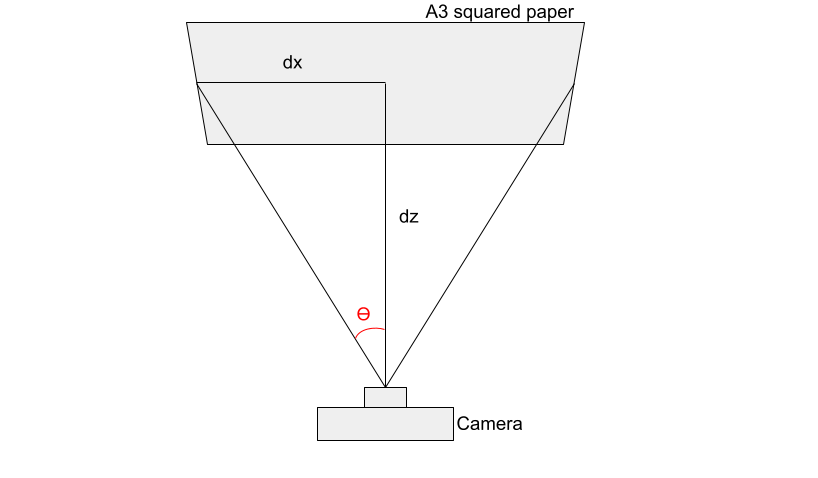
\includegraphics[width=.4\textheight]{Camera_calibration.png}
\captionof{figure}{Figure demonstrating how the calibration angles was calculated}
\label{fig:calib}
\end{figure}

In order to convert pixel positions from footage to the angular position in real space, the conversion must be calibrated to the individual cameras. To achieve this a photograph of A3 squared paper was taken, with the corners of the page just inside the corners of the camera frame. The camera was aligned square to the paper using a spirit level and a plumb wall. The distance from the camera to the wall was recorded using a tape measure. 

The distance from the centre of the photo, assumed to be along a vector normal to the lens, to a point on the squared paper near the edge of the frame was measured in pixels. This distance was also measured in cm using the squares on the paper. 

Using the trigonometric relation of $\tan(\theta)$ the angle from the normal vector to the vector point at B was calculated. Dividing this angle by the pixel distance to B gives the angle per pixel for this camera. This method was repeated for both cameras’ x and y directions.

This technique is very simple to implement, easily repeatable for any camera and is computationally inexpensive. However it is limited in its accuracy due to lens distortions that will change the angle per pixel over the frame. This effectively takes the average angle per pixel and assumes a linear function across the frame.

\subsection{Experimental setup}

\begin{figure}[]
\centering
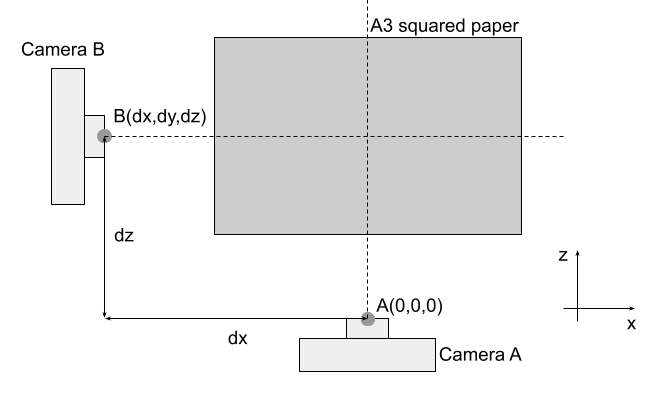
\includegraphics[width=.52\textheight]{Topdown.png}
\captionof{figure}{Experimental set-up}
\label{fig:ex1}
\end{figure}

\begin{figure}[h!]
\centering
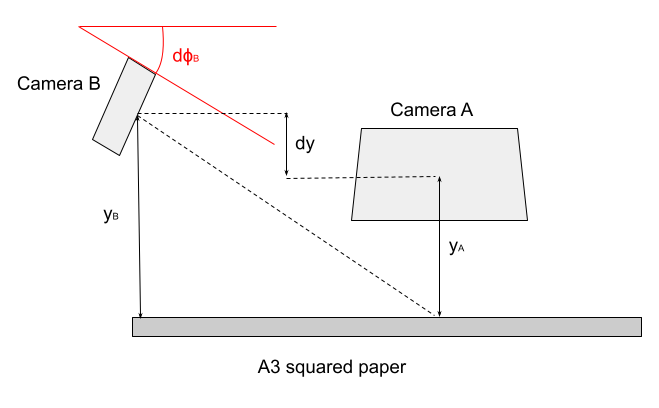
\includegraphics[width=.4\textheight]{Sideon.png}
\captionof{figure}{Experimental set-up}
\label{fig:ex2}
\end{figure}

Figures \ref{fig:ex1}-\ref{fig:ex2} shows our equipment set up, with cameras at points A and B. Initially A3 squared paper was placed in both cameras field of view for testing and validation, however generally this is not necessary. An angle of 90 degrees was used between the cameras so that we gathered the most information on the x and z axis, however using our method the cameras can be at arbitrary points and orientations, so long as they can both see the object, and the angle is measured between them. 

Figure \ref{fig:ex1} shows the x and z measurements that need to be taken between the cameras: $dx$ along the x-axis, which would be negative in this case; and $dz$ along the z-axis, which is positive here. The dotted lines show the centre line of the camera, where the angles for the vectors are calibrated for. 

Figure \ref{fig:ex2} illustrates the side view for our experimental set up. Here it is clearer that the cameras can be angled down, as long as the camera's $d\phi$ is recorded. This angle is shown for camera B in red. This schematic also shows how the height is measured from the floor. The difference is then taken to calculate $dy$, i.e. $dy = \abs{y_B-y_A}$.

 \vspace{5cm}
\subsection{Pre-processing}

Pre-processing of the video footage is vital in order to get accurate results. This section will describe aligning the videos temporally, creating a reference image, finding the difference image, choosing a threshold and using a morphological filter to improve the result. 

\subsubsection{Temporal alignment}

Aligning the videos in time is important so that the vectors calculated for each camera are referring to the object in the same position. Otherwise, the vectors will not converge on the position of the object. This was achieved by switching the lights off and on, and monitoring the average light levels over the frames. By differentiating the curve and looking for the largest gradient, the moment the lights are switched on can be found in each video.
\subsubsection{Gaussian filtering}

A gaussian filter was applied to each frame in the videos to decrease the effect noise has on thresholding. The filter effectively creates a weighted average of pixel intensities in a specified radius for each pixel. This reduces the sharp peaks and troughs of noise intensities, that can evade thresholding. 
 
\subsubsection{Reference image creation}

A reference image is used by the subtraction method to isolate moving objects in a frame, it represents the background of the video, with anything changing then assumed to be the foreground object. Having an object free reference image means that this assumption, bar any noise in the video, will hold true.
 
Two separate ways were explored to create a reference image, taking a clear frame from the video, and averaging the frames over time. Finding a clear frame is preferred over short timescales as this means no artefacts from moving objects in the frame are present. The drawback is that this is a manual process, where the clear frame must be found by eye, before slicing it, and using it for the subtraction images. 

The average method involves meaning all the frames along the time direction, so that each pixel in the final image contains the average intensity of that pixel over the time. This method can be applied automatically and will give a clearer background if no object-free frame can be found. It can also be used to automatically account for lighting condition changes. This can be achieved by updating the reference image using the mean of a subset of frames around the frame of interest. However for a small amount of frames, or where objects do not leave their initial positions for longer than they are in them, it will leave artefacts of the objects at varying intensities. These artefacts may be removed later by the thresholding process, depending on the intensity values left in the reference image. 

\subsubsection{Subtraction image}

The subtraction image is described by equation \ref{eq:eq1}. Where R represents the reference image and f(x,y,t) represents a frame at a point t in time. In our code, the difference before thresholding is calculated first, then thresholding is applied later. Initially, all of the frames are subtracted from the reference image at once, using a reference image that has been repeated into an array at every point in time. The absolute value is taken to ensure that any light level difference, positive or negative are treated the same. In other words a white ball against a black background is equivalent to a black ball on a white one. 

  \begin{equation}
    d_{t}(x,y)
    \begin{cases}
      1, & \text{if}\ \left| R - f(x,y,t) \right| > T \\
      0, & \text{otherwise}
    \end{cases}
    \label{eq:eq1}
  \end{equation}

%\begin{figure}[h!]
%\centering
%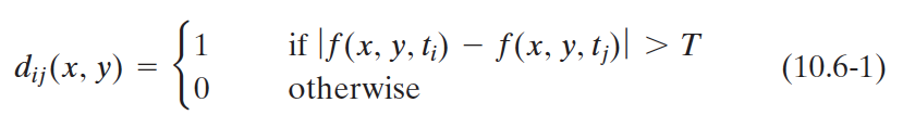
\includegraphics[width=.4\textheight]{Picture1.png}
%\captionof{figure}{\label{fig:eq1}}
%\end{figure}

\subsubsection{Thresholding}

Once the subtraction video has been created, it must be thresholded to remove noise and shadows. This was achieved by first normalising the video so that intensities span the full range of 0 to 1. Then applying a global threshold to every frame which creates a binary mask. This threshold was tuned manually by picking a frame and adjusting so the object is isolated best. 

\subsubsection{Morphological filter}

Due to effects like the reflection of the object, the masks from thresholding often have holes or gaps in, and possibly still some other small artefacts in the frames. We chose to use a closing morphological filter to fill in holes or gaps in the mask. This is a morphological dilation followed by an erosion. The dilation expands the mask at every 1 value by the structuring element, filling in gaps but also overshooting the original edges. The erosion then reduces the size back to the original size.

We used a circular structuring element as this best represented the curved edges expected from the ball. 

\subsection{Finding the coordinates}
The indices of the 1 values were found for the closed masks, then converted to coordinates. The centre of the object in the frame was found by averaging the coordinates and converting to integer values to arrive at the nearest pixel. The pixel positions were then converted into angles in spherical coordinates by multiplying by the conversion factor for each camera found during calibration.

\subsection{Vectors}

The process of mapping an object from a 2D image into 3D space is necessary for tracking a 3D objects using basic cameras. There are cameras which are able to perceive depth. However, they were not used during this project. From the calibration the angle moved through per pixel is calculated. Since the angle per pixel is known, and the centre of mass of the object has been tracked, the number of pixels the COM is from the respective x and y axis are calibrated. The reason why these axes were chosen was to ensure that the 2D image is represented by the x-y axis and the z represents depth. As there are two angles, for the horizontal and vertical displacement respectively, the position of the ball can then be expressed in terms of two polar vectors, which is equivalent to spherical co-ordinates. The Figures \ref{fig:polar} and \ref{fig:sph} show how the vector could be expressed for one plane (xz - horizontal).


\begin{figure}[h!]
\centering
\begin{minipage}{.5\textwidth}
  \centering
  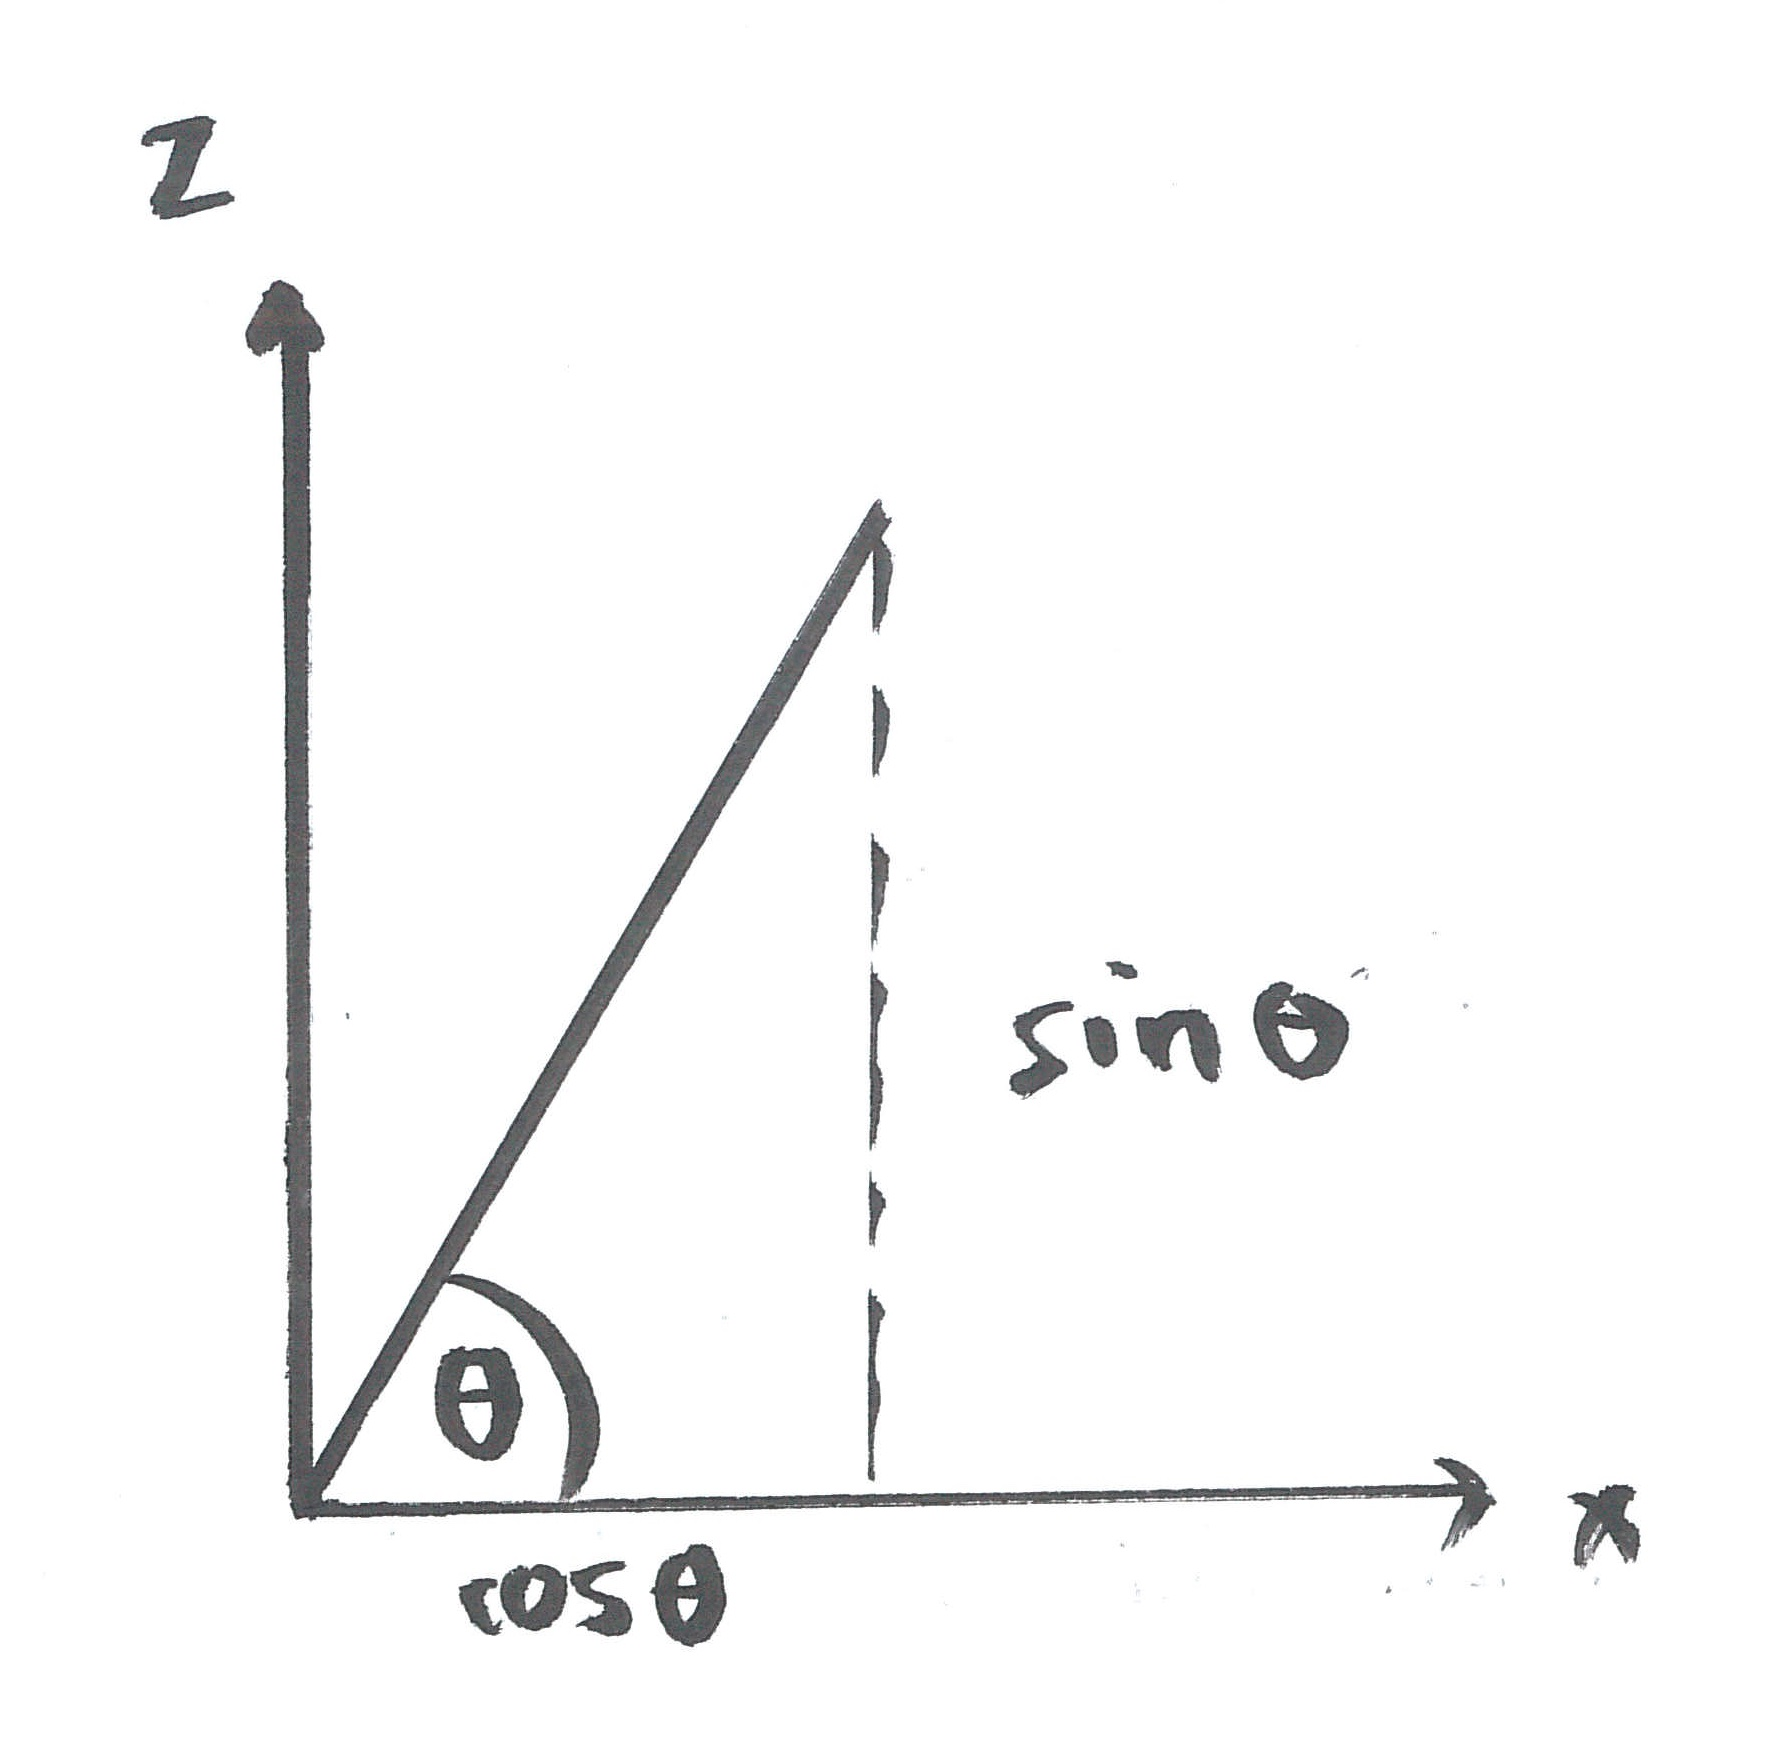
\includegraphics[width=.36\textheight]{Polar.png}
  \captionof{figure}{Polar vector representation on one plane}
  \label{fig:polar}
\end{minipage}%
\begin{minipage}{.5\textwidth}
  \centering
  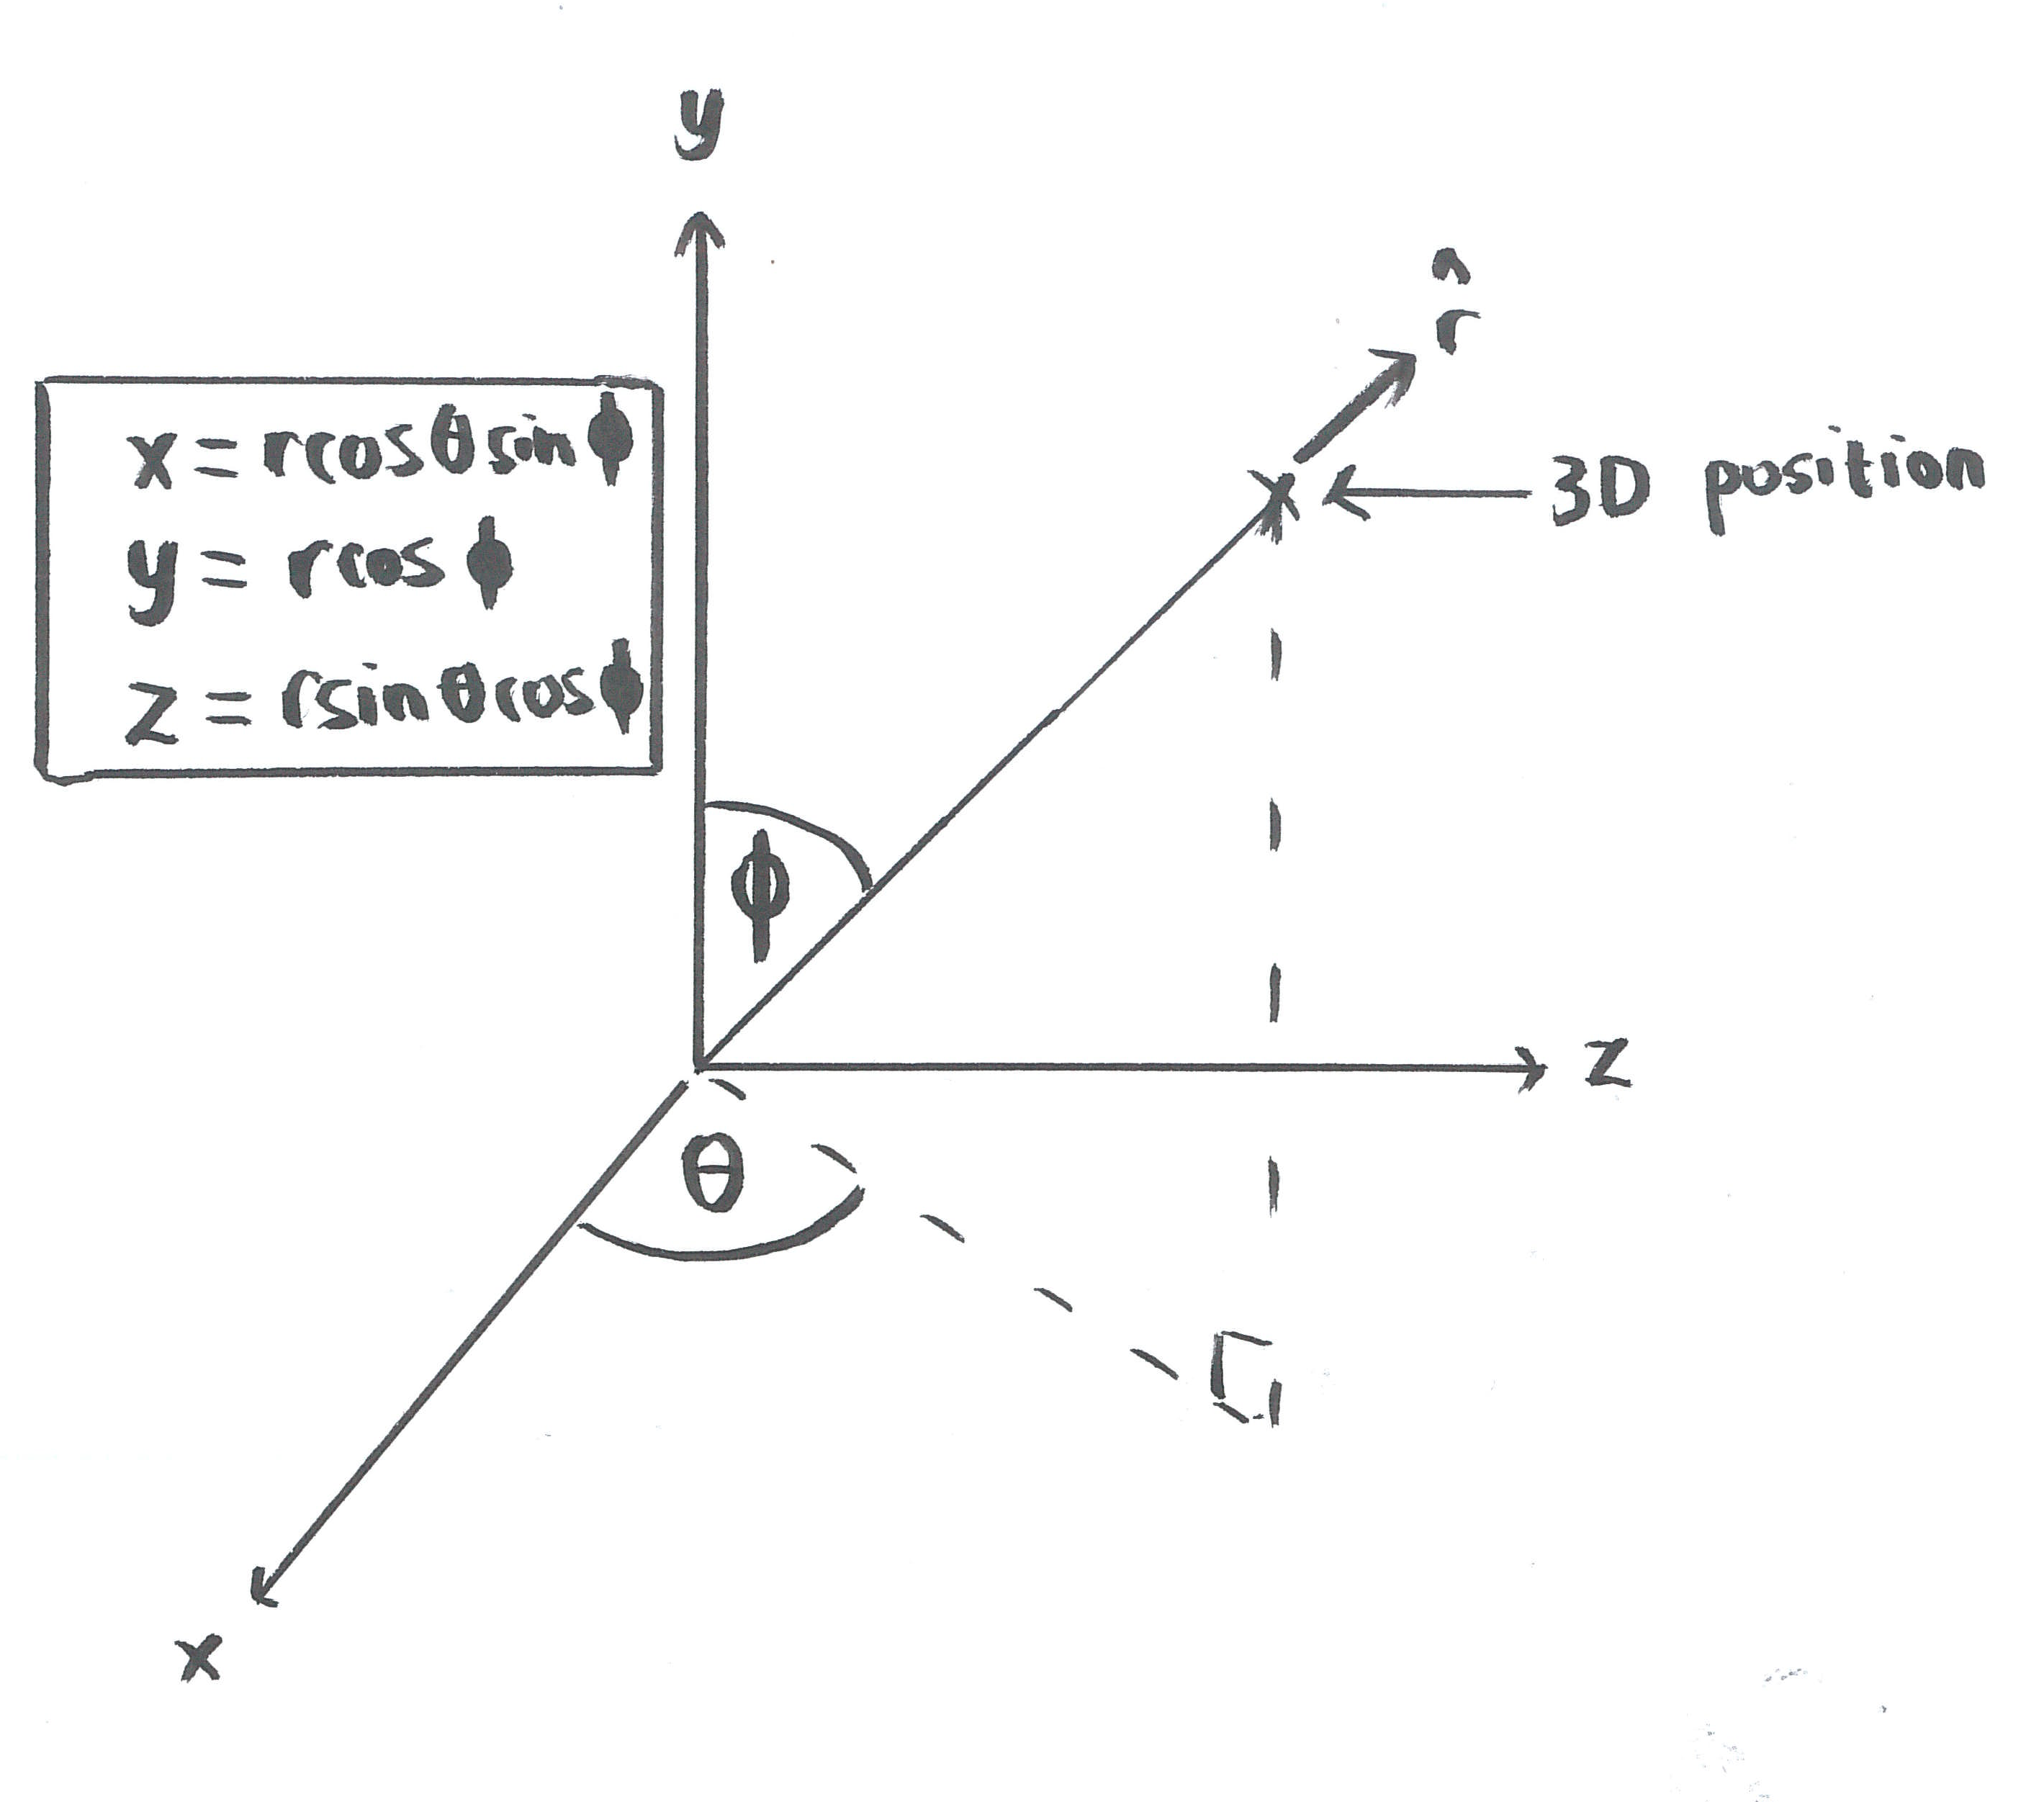
\includegraphics[width=.4\textheight]{Spherical.png}
  \captionof{figure}{Spherical coordinates in 3D}
  \label{fig:sph}
\end{minipage}
\end{figure}

In both of these situations the direction of the vector is known as it is just defined by the two angles, however the value for r (the distance from the camera) is unknown. This is why two vectors are needed so that a value for the depth can be gathered. The vectors gathered will be in the form:

\begin{equation}
	\bf{r} = \begin{bmatrix} r \cos{\theta} \sin{\theta} \\  r \cos{\phi} \\  r \sin{\theta} \sin{\phi} \end{bmatrix} = \begin{bmatrix}
		x \\ y \\ z
	\end{bmatrix}
\end{equation}

The values for theta measured will be that from the normal from the camera to the respective point, therefore they will be measured from a different axis from either camera. However, the axis about which phi is measured will remain the same. With the vector obtained the point at which the vectors are closest to each other needs to be calculated. This point can be calculated using only the vector equations of the lines in cartesian coordinates.

If the two vectors are expressed as such:

\begin{equation}
	\textnormal{Line A: } \ \mathbf{l_A}=\mathbf{r0_A}+\mathbf{v_A} t 
\end{equation}

\begin{equation}
	\textnormal{Line B: } \ \mathbf{l_B}=\mathbf{r0_B}+\mathbf{v_B} t
\end{equation}

The vector perpendicular to these two lines is calculated using the cross product of $\mathbf{v_A}$ and $\mathbf{v_B}$.

\begin{equation}
	\mathbf{n}= \mathbf{v_A} \times \mathbf{v_B}
\end{equation}


The plane which contains $r0_A$ and the translations of Line A is perpendicular to: 

\begin{equation}
	\mathbf{n_B}= \mathbf{v_B} \times \mathbf{n}
\end{equation}

The same is true for $\mathbf{n_B} $ where $\mathbf{n_A}= \mathbf{v_A} \times \mathbf{n}$

The intersecting point of Line A with the above perpendicular plane is given by: 

\begin{equation}
	\mathbf{p_A}=\mathbf{r0_A}+ \frac{(\mathbf{r0_B}-\mathbf{r0_A})\cdot\mathbf{n_B}}{\mathbf{v_A}\cdot\mathbf{n_B}} \mathbf{v_A}
\end{equation}

Similarly, point on Line B nearest to Line A is:

\begin{equation}
	\mathbf{p_B}=\mathbf{r0_B}+ \frac{(\mathbf{r0_A}-\mathbf{r0_B})\cdot\mathbf{n_A}}{\mathbf{v_B}\cdot\mathbf{n_A}} \mathbf{v_B}
\end{equation}

Now, $\mathbf{p_A}$ and $\mathbf{p_B}$ form the shortest line segment joining Line 1 and Line 2.

\newpage

\section{Results}

\begin{figure}[h!] 
  \label{ fig7} 
  \begin{minipage}[b]{0.5\linewidth}
    \centering
    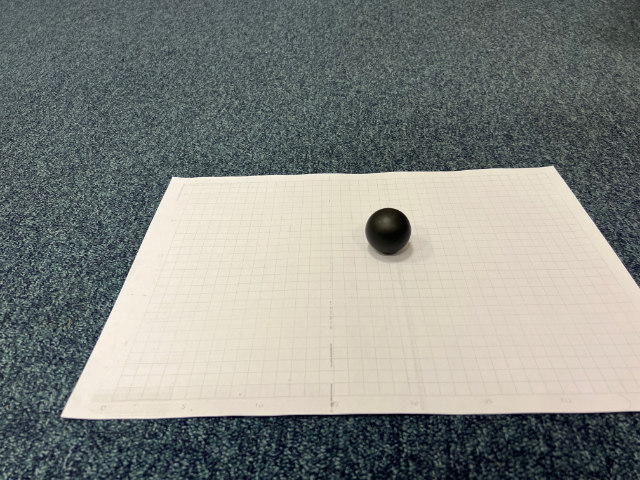
\includegraphics[width=.2\textheight]{1.jpg} 
    \caption{\label{fig:11}Position of ball at [2,-27,34] } 
    \vspace{4ex}
  \end{minipage}%%
  \begin{minipage}[b]{0.5\linewidth}
    \centering
    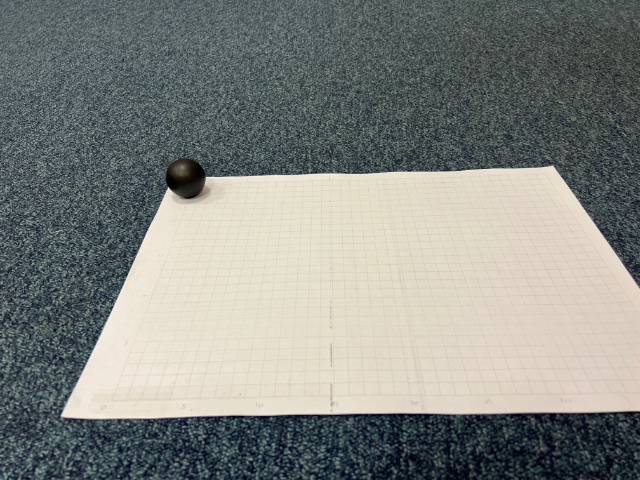
\includegraphics[width=.2\textheight]{2.jpg} 
    \caption{\label{fig:22}Position of ball at [12,-27,54]} 
    \vspace{4ex}
  \end{minipage} 
  \begin{minipage}[b]{0.5\linewidth}
    \centering
    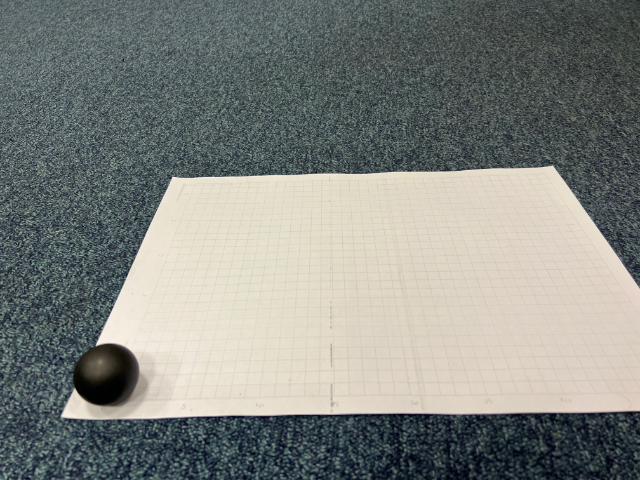
\includegraphics[width=.2\textheight]{3.jpg} 
    \caption{\label{fig:33}Position of ball at [-13,-27,54]} 
    \vspace{4ex}
  \end{minipage}%% 
  \begin{minipage}[b]{0.5\linewidth}
    \centering
    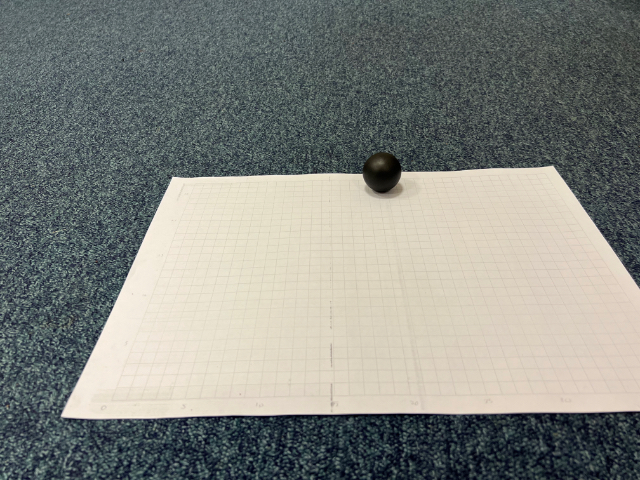
\includegraphics[width=.2\textheight]{4.jpg} 
    \caption{\label{fig:44}Position of ball at [12,-27,34]} 
    \vspace{4ex}
  \end{minipage} 
\end{figure}

\begin{figure}[h!] 
  \label{fig7} 
  \begin{minipage}[b]{0.5\linewidth}
    \centering
    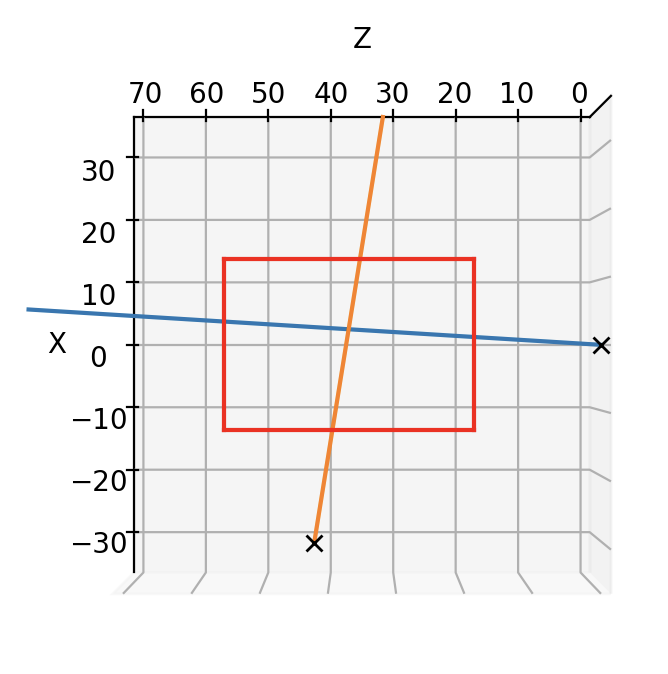
\includegraphics[width=.2\textheight]{11.png} 
    \caption{\label{fig:1}2D vector projection with ball at [2,-27,34]} 
    \vspace{4ex}
  \end{minipage}%%
  \begin{minipage}[b]{0.5\linewidth}
    \centering
    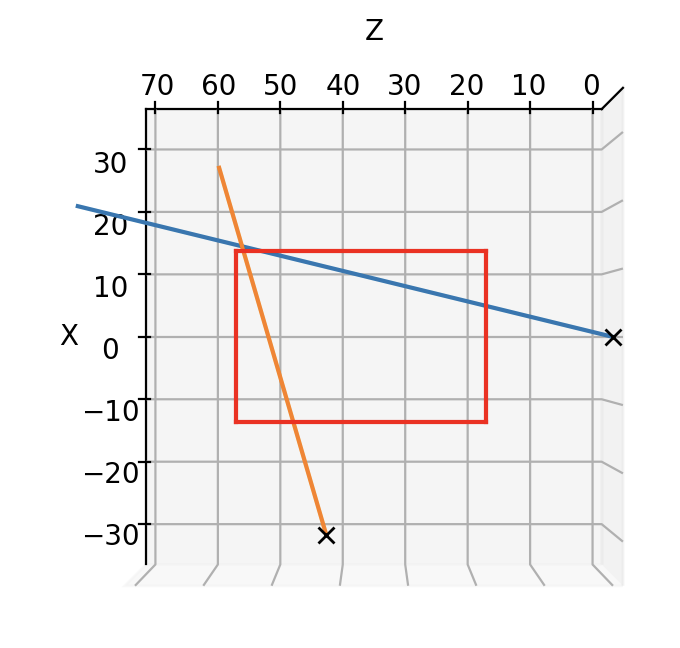
\includegraphics[width=.2\textheight]{22.png} 
    \caption{\label{fig:2}2D vector projection with ball at [12,-27,54]} 
    \vspace{4ex}
  \end{minipage} 
  \begin{minipage}[b]{0.5\linewidth}
    \centering
    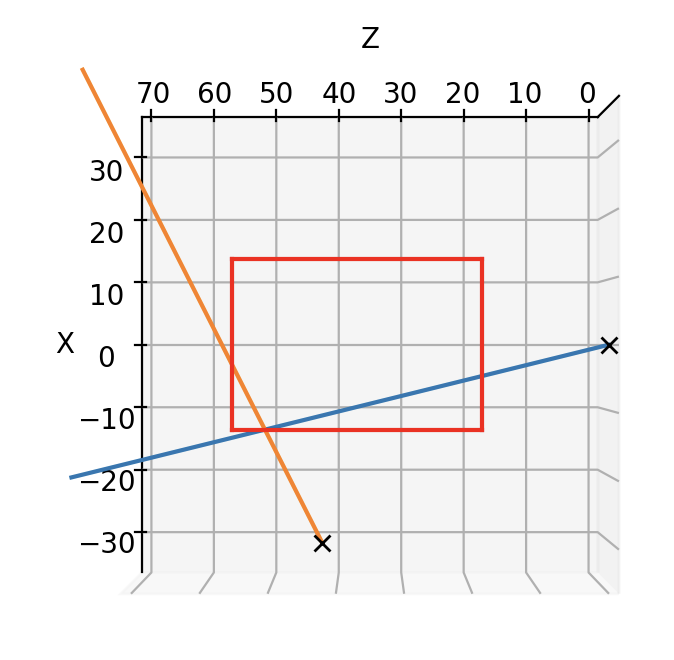
\includegraphics[width=.2\textheight]{33.png} 
    \caption{\label{fig:3}2D vectors projection with ball at [-13,-27,54]} 
    \vspace{4ex}
  \end{minipage}%% 
  \begin{minipage}[b]{0.5\linewidth}
    \centering
    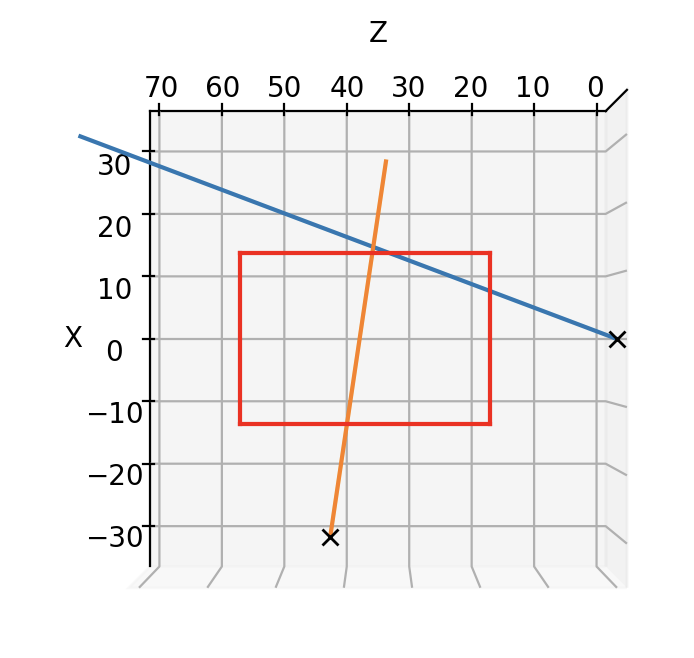
\includegraphics[width=.2\textheight]{44.png} 
    \caption{\label{fig:4}2D vectors projection with ball at [12,-27,34]} 
    \vspace{4ex}
  \end{minipage} 
\end{figure}

\begin{figure}[h!] 
  \label{fig7} 
  \begin{minipage}[b]{0.5\linewidth}
    \centering
    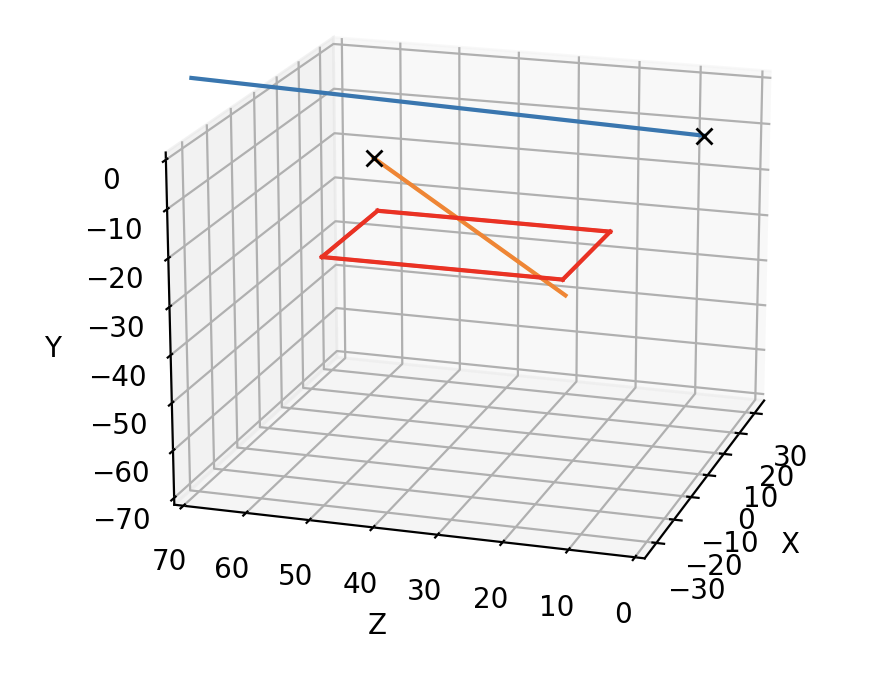
\includegraphics[width=.2\textheight]{111.png} 
    \caption{\label{fig:111}3D vectors projection with ball at [2,-27,34]} 
    \vspace{4ex}
  \end{minipage}%%
  \begin{minipage}[b]{0.5\linewidth}
    \centering
    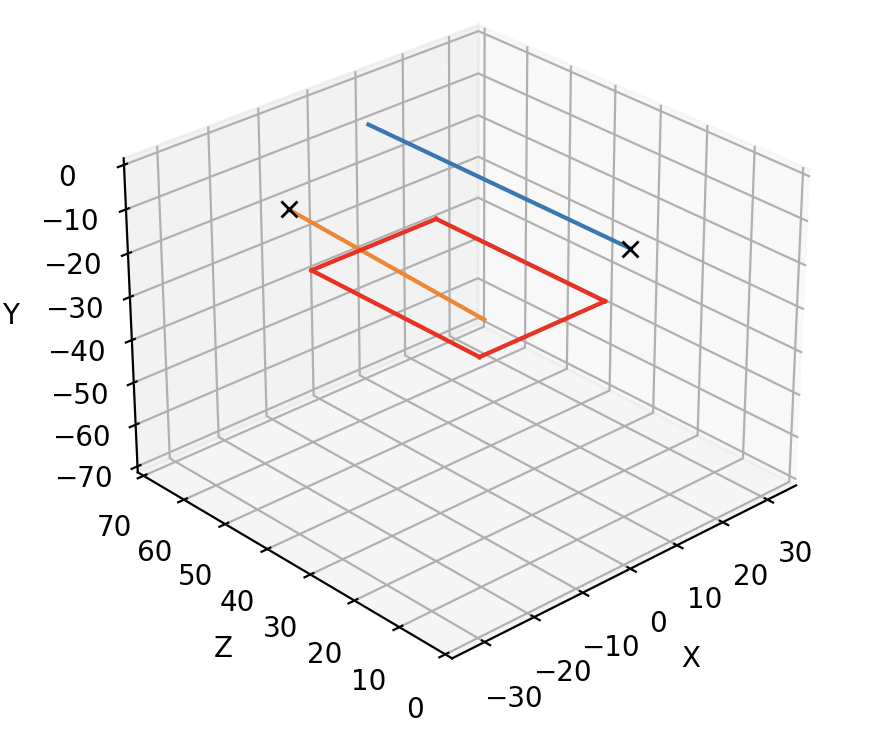
\includegraphics[width=.2\textheight]{222.png} 
    \caption{\label{fig:222}3D vectors projection with ball at [12,-27,54]} 
    \vspace{4ex}
  \end{minipage} 
  \begin{minipage}[b]{0.5\linewidth}
    \centering
    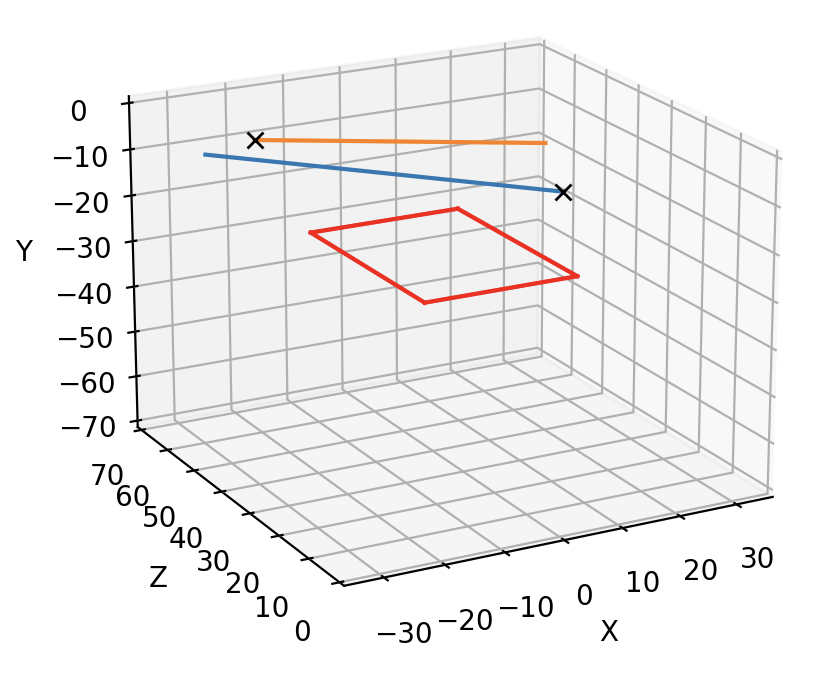
\includegraphics[width=.2\textheight]{333.png} 
    \caption{\label{fig:333}3D vectors projection with ball at [-13,-27,54]} 
    \vspace{4ex}
  \end{minipage}%% 
  \begin{minipage}[b]{0.5\linewidth}
    \centering
    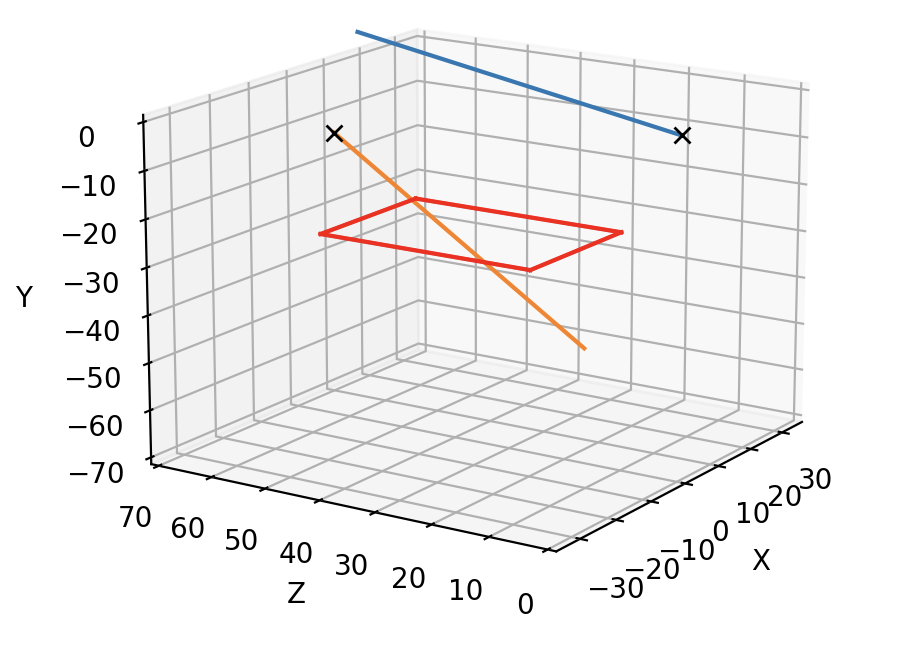
\includegraphics[width=.2\textheight]{444.png} 
    \caption{\label{fig:444}3D vectors projection with ball at [12,-27,34]} 
    \vspace{4ex}
  \end{minipage} 
\end{figure}

\begin{table}[h!]
\centering
\begin{tabular}{c c c c c c c} 
\toprule 
Position of ball & $\Delta x$ (\%) & $\Delta y$ (\%) & Average Error ($\%$)\\[0.5ex] 
\midrule
$[2,34]$ &  $0.16$ & 3.6 & $1.9$\\
$[12, 54]$  & 2.2 & 3.1 & $2.7$\\
$[-13, 54]$ & 8.2 & 5.9 & $7.1$\\
$[12, 54]$ & 10 & 3.4 & $6.7$\\

\midrule
\midrule

Average Error (\%) &  $5.1$ & $4.0$ & $4.6$\\
\end{tabular}
\caption{Difference in percentage of actual position to calculated position}
\label{tab:2D}
\end{table}

$ $

\begin{table}[h!]
\centering
\begin{tabular}{c c c c c c c} 
\toprule 
Position of ball & $\left| \Delta x \right|$ (cm) & $\left| \Delta y  \right|$ (cm) & $\left| \Delta z\right|$ (cm)\\[0.5ex] 
\midrule
$[2, -27, 34]$ &  4.6 & 20 & 23 \\
$[12, -27, 54]$  & 1.8  & 2.3 & 21\\
$[-13, -27, 54]$ & 5.0  & 13 & 21\\
$[12, -27, 34]$ & 7.0  & 18 & 16\\
\midrule
\midrule

$\left| \textnormal{Average Error (cm)} \right|$  & 4.2 & 13 & 21\\
[0.8ex]
%$\textnormal{Standard deviation (cm)} $  & 2.15 &	7.94 &	2.86
$\textnormal{Standard deviation (\%)} $  & 47 & 59 &	14

 
\end{tabular}
\caption{3D position calculated by function LocShortestDistance}
\label{tab:3D}
\end{table}

Figures \ref{fig:1}-\ref{fig:4} show frames captured for validation. These images were taken by camera B in our experimental set up, so the z-axis is pointing from right to left. The x-axis is directed perpendicular to the z-axis, facing out of the camera. In the images the black ball is placed at different locations on the squared paper, with the positions recorded for comparison with our 

Figures \ref{fig:11}-\ref{fig:44} show the 3D vectors calculated using our code for the ball positions in the previous figures. Here the view is shown from the top, approximately showing the projection of the vectors in the x-z plane. The prediction of ball position is represented by where the vector lines cross. The blue line shows the vector from camera A, and the orange line shows the vector from camera B.

Figures \ref{fig:111}-\ref{fig:444} show the vectors in an 3D projection. This shows how the vectors do not cross in 3 dimensions. However a vector position is still calculated from the closest points.

Table \ref{tab:2D} presents the data collected for the 2D projection on the x-z plane. 

Table \ref{tab:3D} presents the positions calculated by our program for each of the ball positions. The absolute error was calculated for each coordinate in x, y and z, then the mean was taken to give the average error for each axis. 

\section{Discussion}

\subsection{Calibration}

Our simple calibration model does not account for the effect of mapping an angle from a point to a 2d flat plane. Figure \ref{fig:lineplot1} shows a plot of lines plotted from the origin, separated by 12\textdegree. Plotting these lines to a straight line perpendicular to the x axis illustrates that the function map is not linear. Greater change of the intersection with the line is seen at larger angles. 

\begin{figure}[h!]
\centering
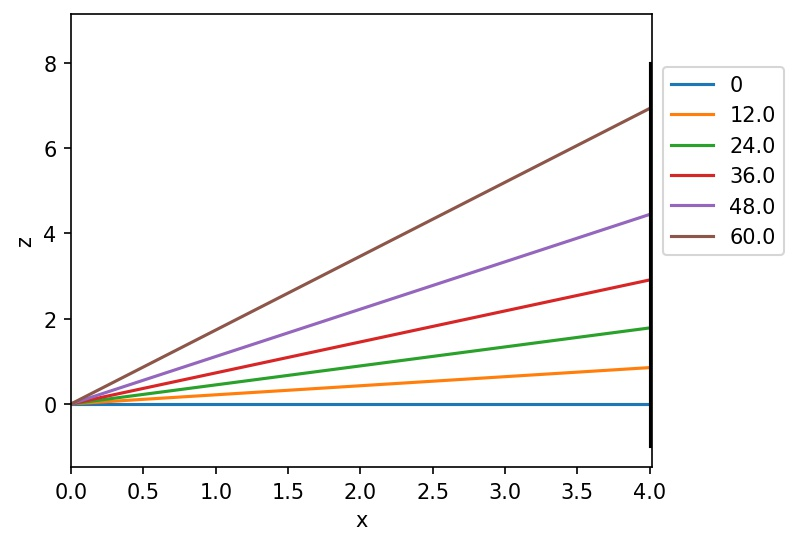
\includegraphics[width=.4\textheight]{lineplot.jpg}
\captionof{figure}{Figure demonstrating how the same angle difference results in differing distances}
\label{fig:lineplot1}
\end{figure}


The calibration could be improved by calculating the angle per pixel for every intersection on the squared paper and creating a function over the 2d space. Multiple repeats would allow for uncertainty to be calculated. 

\subsection{Subtraction method}

The subtraction method works well for moving objects that are distinct from their background. In this paper, grayscale videos were used, however, in a real-life scenario like cricket, colour could be used. To isolate the ball from people moving, a red ball could have been used and by repeating our method in colour-space, just the intense red moving objects could be isolated. This would work, if no other moving objects are red. Another idea could be to use an infrared camera and ignore hot objects like people, however this would not account for the moving bat in cricket. 

\subsection{Thresholding}

The thresholding could be improved by applying different thresholds to each frame, as a global threshold can only be tuned to one frame . Different thresholds could be applied automatically using an algorithm like Otsu’s algorithm. Care must be taken to only threshold frames with the object in. This could be achieved by first using a global threshold, then looping back over the frames with an object in to revise the mask using Otsu’s algorithm. \cite{OTSU}


\subsection{Defining angles}

In this project, angles were defined so that the x and y axis match up with the x and y axis of a photograph. It would have been better to define the axis in line with the maths for spherical coordinates, as this was the most challenging aspect conceptually, which lead to errors in our initial calculations. 

\subsection{Coordinates calculated}
The results in Table\ref{tab:2D} show that our model calculates the position on the x-z plane with an average percentage error of 4.57\%. This is a good result suggesting that our theta angle was calculated with a small error, as this angle describes variation on the x-z plane.

In table \ref{tab:3D} the error for the x-coordinate is low on average, however the standard deviation is very high. This trend is similar with the y-coordinates, with a high standard deviation, although the average error is much higher. The z-coordinates appear to have a consistent error of around 20.5cm, as the standard deviation for these errors is low at 14\%. This suggests a systematic error, however this cannot be confirmed as the phi angle for camera A has such a large systematic error. This is shown in \ref{fig:111}-\ref{fig:444} where it can be seen that the phi angle of vector for camera A is consistently too small. As such it does not intersect camera Bs vector in the correct region. This is likely due to an inaccurate measurement for the initial tilt of the camera. Without correcting for this error, it is impossible to say whether our z-coordinates have a separate error associated with them. 

In the 3D figures, although the angle of camera Bs vectors is mostly intersecting the page, in Figure \ref{fig:333} the phi angle for camera B is very low. After reviewing our calibration images and our video footage, it was found that there was a mismatch in the pixel sizes for the frames. This may account for some of the error found in both cameras phi angles. Recollection of the verification pictures would be needed to confirm our error sources. 

\subsection{Future developments}
Currently the calibration of the cameras is manual, and does not take into account the problems of mapping an angle to a flat plane and distortion from the camera lens. In the future ChArUco, a chessboard with unique patterns on each square, could be used. Then a function could be written such that the only manual input needed would be taking the pictures of the ChArUco. The function would map the positions of the cameras in 3D space and calibrate them automatically. This would remove the majority of the manual data collection during the experiment, and allow for the system to be deployed with greater ease. 

Another opportunity for future development is the segmentation of the object. Currently this is accomplished by a simple subtraction model, however this makes the often wrong assumption that everything changing in the frame is the object being tracked. Both colour segmentation or infrared data collection could improve this result, however, training a convolutional neural network may be a more robust technique to dealing with confounding factors in the frame.\cite{CNN} 


\section{Conclusion}
This project outlined the creation of a rudimentary version of Hawkeye. Our results showed a good level of accuracy in a 2D plane, with an average percentage error of 4.6\%. However the same accuracy was not replicated in 3 dimensions, due to the systematic error in camera As delta phi measurement, in conjunction with a likely error in calibration of the angles within our script. 

The procedure we have developed and outlined here, forms a good foundation for further developments to expand upon. We make this freely available to the world. 



\begin{thebibliography}{9}
\bibitem{OTSU}
OTSUs method: Rafael C. Gonzalez, Richard E. Woods, “Digital Image Processing”, Second Edition, ISBN 0-201-18075-8.

\bibitem{FOXTENN}
Foxtenn.com. 2021. [online] Available at: http://www.foxtenn.com/in\&out [Accessed 9 November 2021].

\bibitem{CNN}
P.R. Kamble, A.G. Keskar, K.M. Bhurchandi,
A deep learning ball tracking system in soccer videos,
Opto-Electronics Review,
Volume 27, Issue 1,
2019,
Pages 58-69,
ISSN 1230-3402,



\bibitem{1}
T. Qazi, P. Mukherjee, S. Srivastava, B. Lall and N. R. Chauhan, ”Automated ball tracking in tennis videos,” 2015 Third Interna- tional Conference on Image Information Processing (ICIIP), Wak- naghat, 2015, pp. 236-240, http://ieeexplore.ieee.org/ document/7414772/
\bibitem{2}
C. Lyu, Y. Liu, B. Li and H. Chen, ”Multi-feature based high-speed ball shape target tracking,” 2015 IEEE International Conference on Information and Automation, Lijiang, 2015, pp. 67-72. doi: 10.1109/ICInfA.2015.7279260
\bibitem{4}
Yan, F, Christmas, W and Kittler, J (2005) A Tennis Ball Tracking Algorithm for Automatic Annotation of Tennis Match In: British Machine Vision Conference, 2005-09-05 - 2005-09-08, Oxford, UK.
\bibitem{5}
B. Ekinci, M. Gokmen, ”A ball tracking system for offline ten- nis videos”, International Conference on Visualization Imaging and Simulation 2008, http://www.wseas.us/e- library/ conferences/2008/bucharest2/vis/vis06.pdf


\end{thebibliography}


\end{document}

